\documentclass[12pt, oneside]{article}

\usepackage[letterpaper, scale=0.89, centering]{geometry}
\usepackage{fancyhdr}
\setlength{\parindent}{0em}
\setlength{\parskip}{1em}

\pagestyle{fancy}
\fancyhf{}
\renewcommand{\headrulewidth}{0pt}
\rfoot{\href{https://creativecommons.org/licenses/by-nc-sa/2.0/}{CC BY-NC-SA 2.0} Version \today~(\thepage)}

\usepackage{amssymb,amsmath,pifont,amsfonts,comment,enumerate,enumitem}
\usepackage{currfile,xstring,hyperref,tabularx,graphicx,wasysym}
\usepackage[labelformat=empty]{caption}
\usepackage[dvipsnames,table]{xcolor}
\usepackage{multicol,multirow,array,listings,tabularx,lastpage,textcomp,booktabs}

\lstnewenvironment{algorithm}[1][] {   
    \lstset{ mathescape=true,
        frame=tB,
        numbers=left, 
        numberstyle=\tiny,
        basicstyle=\rmfamily\scriptsize, 
        keywordstyle=\color{black}\bfseries,
        keywords={,procedure, div, for, to, input, output, return, datatype, function, in, if, else, foreach, while, begin, end, }
        numbers=left,
        xleftmargin=.04\textwidth,
        #1
    }
}
{}
\lstnewenvironment{java}[1][]
{   
    \lstset{
        language=java,
        mathescape=true,
        frame=tB,
        numbers=left, 
        numberstyle=\tiny,
        basicstyle=\ttfamily\scriptsize, 
        keywordstyle=\color{black}\bfseries,
        keywords={, int, double, for, return, if, else, while, }
        numbers=left,
        xleftmargin=.04\textwidth,
        #1
    }
}
{}

\newcommand\abs[1]{\lvert~#1~\rvert}
\newcommand{\st}{\mid}

\newcommand{\A}[0]{\texttt{A}}
\newcommand{\C}[0]{\texttt{C}}
\newcommand{\G}[0]{\texttt{G}}
\newcommand{\U}[0]{\texttt{U}}

\newcommand{\cmark}{\ding{51}}
\newcommand{\xmark}{\ding{55}}
 
\begin{document}
\begin{flushright}
    \StrBefore{\currfilename}{.}
\end{flushright} \section*{Week5 monday}


To fully specify a PDA we could give its $6$-tuple formal definition or we could give its input 
alphabet, stack alphabet, and state diagram.
An informal description of a PDA is a step-by-step description of how its computations 
would process input strings; the reader should be able to reconstruct the state diagram or formal 
definition precisely from such a descripton. The informal description of a PDA can refer to some 
common modules or subroutines that are computable by PDAs:
\begin{itemize}
  \item PDAs can ``test for emptyness of stack'' without providing details. 
  {\it How?} We can always push a special end-of-stack symbol, $\$$, at the start, before processing
  any input, and then use this symbol as a flag.
  \item PDAs can ``test for end of input'' without providing details.
  {\it How?} We can transform a PDA to one where accepting states are only those reachable 
  when there are no more input symbols.
\end{itemize}

{\it Big picture}: PDAs were motivated by wanting to add some memory of unbounded size to NFA. How 
do we accomplish a similar enhancement of regular expressions to get a syntactic model that is 
more expressive?

DFA, NFA, PDA: Machines process one input string at a time; the computation of a machine on its input string 
reads the input from left to right.

Regular expressions: Syntactic descriptions of all strings that match a particular pattern; the language 
described by a regular expression is built up recursively according to the expression's syntax

{\bf Context-free grammars}: Rules to produce one string at a time, adding characters from the middle, beginning, 
or end of the final string as the derivation proceeds.


\begin{center}
  \hspace{-0.25in}\begin{tabular}{|p{2in}cp{4in}|}
  \hline 
  Term & Typical symbol & Definition \\
  \hline\hline
  {\bf Context-free grammar} (CFG) & $G$ & $G = (V, \Sigma, R, S)$ \\
  {\bf Variables}& $V$ & Finite  set of symbols that represent phases in production pattern\\
  {\bf Terminals} & $\Sigma$ & Alphabet of symbols of strings generated  by CFG \\
  & & $V \cap \Sigma = \emptyset$ \\
  {\bf Rules}& $R$ & Each rule is  $A \to u$ with $A \in V$ and $u  \in (V  \cup \Sigma)^*$\\
  Start variable&  $S$  & Usually  on LHS of first / topmost rule \\
  {\bf Derivation} & & Sequence  of substitutions in a  CFG \\
  & $S \implies \cdots \implies w$ & Start with start variable, apply one rule to one occurrence of a variable at a time\\
  {\bf Language} generated by the CFG $G$ & $L(G)$ &$\{  w \in \Sigma^* \mid \text{there is  derivation in $G$ that ends
  in $w$} \} = \{  w \in \Sigma^* \mid S \implies^* w \}$\\
  {\bf Context-free language} & & A language that is the language generated by some CFG\\
  \hline
  Sipser pages 102-103 & &\\
  \hline
  \end{tabular}
  \end{center}
  
{\bf Examples of context-free grammars, derivations in those grammars, and the languages generated by those grammars}
  
$G_1 =  (\{S\}, \{0\}, R, S)$ with rules
  \begin{align*}
    &S \to 0S\\
    &S \to 0\\
  \end{align*}
  In  $L(G_1)$ \ldots 
  
  \vspace{110pt}
  
  Not in $L(G_1)$ \ldots 

  \vspace{110pt}


  $G_2 =  (\{S\}, \{0,1\}, R, S)$
  \[
  S \to 0S \mid 1S \mid \varepsilon
  \]
  In  $L(G_2)$ \ldots 
  
  \vspace{110pt}
  
  Not in $L(G_2)$ \ldots 

  \vspace{110pt}

  $(\{S, T\}, \{0, 1\}, R, S)$ with  rules
  \begin{align*}
  &S \to T1T1T1T \\
  &T \to  0T \mid 1T \mid \varepsilon
  \end{align*}

  In  $L(G_3)$ \ldots 
  
  \vspace{110pt}
  
  Not in $L(G_3)$ \ldots 

  \vspace{110pt}


  $G_4 =  (\{A, B\}, \{0, 1\}, R, A)$ with rules
  \[
    A \to 0A0 \mid  0A1 \mid 1A0  \mid 1A1 \mid  1
  \]
  In  $L(G_4)$ \ldots 
  
  \vspace{110pt}
  
  Not in $L(G_4)$ \ldots 

  \vspace{110pt}

  
{\it Extra practice}: Is there a CFG $G$ with $L(G) = \emptyset$?

  \newpage
  
  Design a CFG to generate the  language $\{abba\}$
  
  \begin{align*}
  & ( \{ S, T, V, W\}, \{a,b\}, \{ S \to aT, T \to bV, V \to bW, W \to a\}, S)\\
  & \\ 
  & \\ 
  & \\ 
  & ( \{ Q \}, \{a,b\}, \{Q \to abba\}, Q) \\
  & \\ 
  & \\ 
  & \\
  & ( \{ X,Y \}, \{a,b\}, \{X \to aYa, Y \to bb\}, X) 
  & \\ 
  & \\ 
  \end{align*} 


  Design a CFG to generate the  language $\{a^n b^n \mid  n  \geq  0\}$
  
  \vspace{150pt}
  
  {\it Sample derivation:} 
  
  \vspace{30pt}
  
  
  Design a CFG to generate the  language $\{a^i b^j \mid j \geq i  \geq 0\}$
  
  \vspace{150pt}
  
  {\it Sample derivation:} 
  
  \vspace{30pt}
 \vfill
\section*{Week5 wednesday}


{\bf Theorem  2.20}: A language is  generated by some context-free  grammar
if  and only if it is recognized by some push-down automaton.

Definition: a language is called {\bf context-free} if it is the language generated by a context-free grammar.
The class of all context-free language over a given alphabet $\Sigma$ is called {\bf CFL}.

Consequences:
\begin{itemize}
    \item Quick proof that every regular language is context free 
    \item To prove closure of the class of context-free languages under a given operation, we can choose 
    either of two modes 
    of proof (via CFGs or PDAs) depending on which is easier
\end{itemize}


Over $\Sigma = \{a,b\}$, let $L = \{ a^n b^m \mid n  \neq m \}$. {\bf Goal}: Prove $L$ is context-free.


\vfill

\newpage
Suppose $L_1$ and $L_2$ are context-free languages over $\Sigma$.  {\bf Goal}:  $L_1 \cup L_2$  is  also context-free.

{\it Approach 1: with  PDAs}

Let $M_1 = ( Q_1, \Sigma, \Gamma_1, \delta_1, q_1, F_1)$ and
$M_2 = ( Q_2, \Sigma, \Gamma_2, \delta_2, q_2, F_2)$ be PDAs with 
$L(M_1) =  L_1$  and  $L(M_2) = L_2$.

Define $M = $

\vfill

{\it Approach  2: with CFGs}

Let $G_1 = (V_1, \Sigma, R_1, S_1)$  and   $G_2 = (V_2, \Sigma, R_2, S_2)$  be CFGs  with
$L(G_1) =  L_1$  and  $L(G_2) = L_2$.

Define $G = $

\vfill

\newpage
Suppose $L_1$ and $L_2$ are context-free languages over $\Sigma$.  {\bf Goal}:  $L_1 \circ L_2$  is  also context-free.


{\it Approach 1: with  PDAs}

Let $M_1 = ( Q_1, \Sigma, \Gamma_1, \delta_1, q_1, F_1)$ and
$M_2 = ( Q_2, \Sigma, \Gamma_2, \delta_2, q_2, F_2)$ be PDAs with 
$L(M_1) =  L_1$  and  $L(M_2) = L_2$.

Define $M = $

\vfill

{\it Approach  2: with CFGs}

Let $G_1 = (V_1, \Sigma, R_1, S_1)$  and   $G_2 = (V_2, \Sigma, R_2, S_2)$  be CFGs  with
$L(G_1) =  L_1$  and  $L(G_2) = L_2$.

Define $G = $

\vfill
\newpage
{\it Summary}

Over a fixed alphabet $\Sigma$, a language $L$ is {\bf regular}

\vspace{-20pt}
\begin{center}
    iff it is described by some regular expression \\
    iff it is recognized by some DFA\\
    iff it is recognized by some NFA
\end{center}

Over a fixed alphabet $\Sigma$, a language $L$ is {\bf context-free}

\vspace{-20pt}
\begin{center}
    iff it is generated by some CFG\\
    iff it is recognized by some PDA
\end{center}

{\bf Fact}: Every regular language is a context-free language.

{\bf Fact}: There are context-free languages that are not nonregular.

{\bf Fact}: There are countably many regular languages.

{\bf Fact}: There are countably inifnitely many context-free languages.

{\it Consequence}: Most languages are {\bf not} context-free!

{\bf Examples  of non-context-free languages}

\begin{align*}
    &\{ a^n b^n c^n \mid 0 \leq n , n \in \mathbb{Z}\}\\
    &\{ a^i b^j c^k \mid 0 \leq i \leq j \leq k , i \in \mathbb{Z}, j \in \mathbb{Z}, k \in \mathbb{Z}\}\\
    &\{ ww \mid w \in \{0,1\}^* \}
\end{align*}
(Sipser Ex 2.36, Ex 2.37, 2.38)

There is a Pumping Lemma for CFL that can be used to prove a specific language is non-context-free: 
If $A$ is a context-free language, there there
is a number $p$ where, if $s$ is any string in $A$ of length at least $p$, then $s$ may be divided 
into five pieces $s = uvxyz$ where (1) for each $i \geq 0$, $uv^ixy^iz \in A$, (2) $|uv|>0$, (3) $|vxy| \leq p$.
{\it We will not go into the details of the proof or application of Pumping Lemma for CFLs this quarter.} \vfill
\section*{Week5 friday}


A set $X$ is said to be {\bf closed} under an operation $OP$ if, for any elements in $X$, applying 
$OP$ to them gives an element in $X$.  


\begin{center}
\begin{tabular}{|c|l|}
\hline
True/False & Closure claim \\
\hline
True &  The set of integers is closed under multiplication. \\
& $\forall x \forall y \left( ~(x \in \mathbb{Z} \wedge y \in \mathbb{Z})\to xy \in \mathbb{Z}~\right)$ \\
\hline
True & For each set $A$, the power set of $A$ is closed under intersection. \\
& $\forall A_1 \forall A_2 \left( ~(A_1 \in \mathcal{P}(A) \wedge A_2 \in \mathcal{P}(A) \in \mathbb{Z}) \to A_1 \cap A_2 \in \mathcal{P}(A)~\right)$ \\
\hline
  & The class of regular languages over $\Sigma$ is closed under complementation. \\
  & \\
 \hline
  & The class of regular languages over $\Sigma$ is closed under union. \\
  & \\
 \hline
  & The class of regular languages over $\Sigma$ is closed under intersection. \\
  & \\
  \hline
  & The class of regular languages over $\Sigma$ is closed under concatenation. \\
  & \\
 \hline
  & The class of regular languages over $\Sigma$ is closed under Kleene star. \\
  & \\
\hline
    & The class of context-free languages over $\Sigma$ is closed under complementation. \\
  & \\
\hline
    & The class of context-free languages over $\Sigma$ is closed under union. \\
  & \\
\hline
    & The class of context-free languages over $\Sigma$ is closed under intersection. \\
  & \\
\hline
    & The class of context-free languages over $\Sigma$ is closed under concatenation. \\
  & \\
\hline
    & The class of context-free languages over $\Sigma$ is closed under Kleene star. \\
  & \\
\hline
\end{tabular}
\end{center}

\vfill

Assume  $\Sigma  = \{0,1, \#\}$
\begin{center}
\begin{tabular}{|cc|}
\hline
&\\
$\Sigma^*$  & Regular ~~/~~ nonregular and context-free ~~/~~not context-free\\

$\{0^i\# 1^j \mid i \geq  0, j  \geq 0\}$  & Regular ~~/~~ nonregular and context-free ~~/~~not context-free\\

$\{0^i1^j\# 1^j0^i \mid i \geq  0, j  \geq 0\}$  & Regular ~~/~~ nonregular and context-free ~~/~~not context-free\\

$\{0^i1^j\# 0^i 1^j \mid i \geq  0, j  \geq 0\}$  & Regular ~~/~~ nonregular and context-free ~~/~~not context-free\\
&\\
\hline
\end{tabular}
\end{center}

\newpage
{\bf Turing machines}: unlimited read + write memory, unlimited time (computation can proceed
without ``consuming'' input and can re-read symbols of input)
\begin{itemize}
\item Division betweeen program (CPU, state diagram) and data
\item Unbounded memory gives theoretical limit to what modern computation 
(including PCs, supercomputers, quantum computers) can achieve
\item State diagram formulation is simple enough to reason about (and diagonalize against) while
expressive enough to capture modern computation
\end{itemize}

For Turing machine $M= (Q, \Sigma, \Gamma, \delta, q_0, q_{accept}, q_{reject})$ 
the {\bf computation} of $M$ on a string $w$ over $\Sigma$  is:

\vspace{-20pt}

\begin{itemize}
\setlength{\itemsep}{0pt}
\item Read/write head starts at leftmost position on tape. 
\item Input string is written on $|w|$-many leftmost cells of tape, 
rest of  the tape cells have  the blank symbol. {\bf Tape alphabet} 
is $\Gamma$ with $\textvisiblespace\in \Gamma$ and $\Sigma \subseteq \Gamma$.
The blank symbol $\textvisiblespace \notin \Sigma$.
\item Given current state of machine and current symbol being read at the tape head, 
the machine transitions to next state, writes a symbol to the current position  of the 
tape  head (overwriting existing symbol), and moves the tape head L or R (if possible). 
Formally, {\bf transition function}  is 
\[
  \delta: Q\times \Gamma \to Q \times \Gamma \times \{L, R\}
\]
\item Computation ends if and when machine enters either the accept or the reject state.
This is called {\bf halting}.
Note: $q_{accept} \neq q_{reject}$.
\end{itemize}

The {\bf language recognized by the  Turing machine} $M$,  is  
\[
  \{ w \in \Sigma^* \mid \textrm{computation of $M$ on $w$ halts after entering the accept state}\} = \{ w \in \Sigma^* \mid w \textrm{ is accepted by } M\}
\]

\newpage
An example Turing machine: $\Sigma = \phantom{\hspace{1in}}, \Gamma = \phantom{\hspace{1in}} $
\[
  \delta ( ( q0, 0)  ) =  
\]

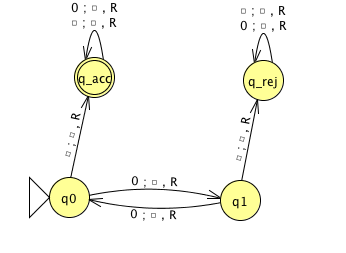
\includegraphics[width=2.5in]{resources/machines/Lect13TM1.png}

Formal definition: 


Sample computation: 

\begin{tabular}{|c|c|c|c|c|c|c|}
\hline
\multicolumn{1}{|c}{$q0\downarrow$} &  \multicolumn{6}{c|}{\phantom{A}}\\
\hline
$0$ & $0$  & $0$ & $\textvisiblespace $& $\textvisiblespace $& $\textvisiblespace $&  $\textvisiblespace $\\
\hline
\multicolumn{7}{|c|}{\phantom{A}}\\
\hline
\phantom{AA} & \phantom{AA}& \phantom{AA}& \phantom{AA}& \phantom{AA}& \phantom{AA}& \phantom{AA} \\
\hline
\multicolumn{7}{|c|}{\phantom{A}}\\
\hline
\phantom{AA} & \phantom{AA}& \phantom{AA}& \phantom{AA}& \phantom{AA}& \phantom{AA}& \phantom{AA} \\
\hline
\multicolumn{7}{|c|}{\phantom{A}}\\
\hline
\phantom{AA} & \phantom{AA}& \phantom{AA}& \phantom{AA}& \phantom{AA}& \phantom{AA}& \phantom{AA} \\
\hline
\multicolumn{7}{|c|}{\phantom{A}}\\
\hline
\phantom{AA} & \phantom{AA}& \phantom{AA}& \phantom{AA}& \phantom{AA}& \phantom{AA}& \phantom{AA} \\
\hline
\end{tabular}

\vfill

The language recognized by this machine is \ldots

{\it Extra practice:}

 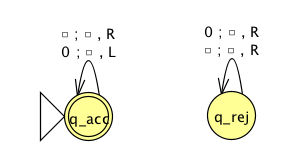
\includegraphics[width=2in]{resources/machines/Lect13TM2.png} 


 Formal definition: 


 Sample computation: 
 

\newpage
{\it Sipser Figure  3.10}

{\bf Conventions in state diagram of TM}: $b \to R$ label means $b \to b, R$ and
all arrows missing from diagram represent transitions with output $(q_{reject}, \textvisiblespace , R)$

\begin{multicols}{2}
\vspace{-20pt}
\begin{center}
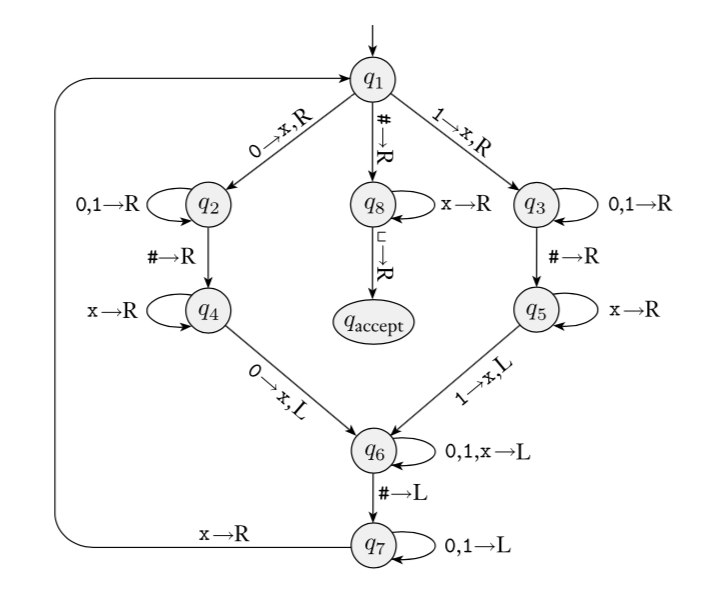
\includegraphics[width=4in]{resources/machines/Lect13TM3.png}
\end{center}

Implementation level description of this machine:
\begin{quote}
Zig-zag across tape to corresponding positions on either side of $\#$ to check whether the 
characters in these positions agree. If they do not, or if there is no $\#$, reject. If they 
do, cross them off.

Once all symbols to the left of the $\#$ are crossed off, check for any un-crossed-off symbols 
to the right of $\#$; if there are any, reject; if there aren't, accept.
\end{quote}

\columnbreak

Computation on  input  string  $01\#01$

\begin{tabular}{|c|c|c|c|c|c|c|}
\hline
\multicolumn{1}{|c}{$q_1 \downarrow$} &  \multicolumn{6}{c|}{\phantom{A}}\\
\hline
$0$ & $1$  & $\#$  & $0$ & $1$ & $\textvisiblespace $& $\textvisiblespace $\\
\hline
  \multicolumn{7}{|c|}{\phantom{A}}\\
  \hline
  \phantom{AA} & \phantom{AA}& \phantom{AA}& \phantom{AA}& \phantom{AA}& \phantom{AA}& \phantom{AA} \\
  \hline
  \multicolumn{7}{|c|}{\phantom{A}}\\
  \hline
  \phantom{AA} & \phantom{AA}& \phantom{AA}& \phantom{AA}& \phantom{AA}& \phantom{AA}& \phantom{AA} \\
  \hline
  \multicolumn{7}{|c|}{\phantom{A}}\\
  \hline
  \phantom{AA} & \phantom{AA}& \phantom{AA}& \phantom{AA}& \phantom{AA}& \phantom{AA}& \phantom{AA} \\
  \hline
  \multicolumn{7}{|c|}{\phantom{A}}\\
  \hline
  \phantom{AA} & \phantom{AA}& \phantom{AA}& \phantom{AA}& \phantom{AA}& \phantom{AA}& \phantom{AA} \\
  \hline
  \multicolumn{7}{|c|}{\phantom{A}}\\
  \hline
  \phantom{AA} & \phantom{AA}& \phantom{AA}& \phantom{AA}& \phantom{AA}& \phantom{AA}& \phantom{AA} \\
  \hline
  \multicolumn{7}{|c|}{\phantom{A}}\\
  \hline
  \phantom{AA} & \phantom{AA}& \phantom{AA}& \phantom{AA}& \phantom{AA}& \phantom{AA}& \phantom{AA} \\
  \hline
  \multicolumn{7}{|c|}{\phantom{A}}\\
  \hline
  \phantom{AA} & \phantom{AA}& \phantom{AA}& \phantom{AA}& \phantom{AA}& \phantom{AA}& \phantom{AA} \\
  \hline
  \multicolumn{7}{|c|}{\phantom{A}}\\
  \hline
  \phantom{AA} & \phantom{AA}& \phantom{AA}& \phantom{AA}& \phantom{AA}& \phantom{AA}& \phantom{AA} \\
  \hline
  \multicolumn{7}{|c|}{\phantom{A}}\\
  \hline
  \phantom{AA} & \phantom{AA}& \phantom{AA}& \phantom{AA}& \phantom{AA}& \phantom{AA}& \phantom{AA} \\
  \hline
  \multicolumn{7}{|c|}{\phantom{A}}\\
  \hline
  \phantom{AA} & \phantom{AA}& \phantom{AA}& \phantom{AA}& \phantom{AA}& \phantom{AA}& \phantom{AA} \\
  \hline
  \multicolumn{7}{|c|}{\phantom{A}}\\
  \hline
  \phantom{AA} & \phantom{AA}& \phantom{AA}& \phantom{AA}& \phantom{AA}& \phantom{AA}& \phantom{AA} \\
  \hline
  \multicolumn{7}{|c|}{\phantom{A}}\\
  \hline
  \phantom{AA} & \phantom{AA}& \phantom{AA}& \phantom{AA}& \phantom{AA}& \phantom{AA}& \phantom{AA} \\
  \hline
  \multicolumn{7}{|c|}{\phantom{A}}\\
  \hline
  \phantom{AA} & \phantom{AA}& \phantom{AA}& \phantom{AA}& \phantom{AA}& \phantom{AA}& \phantom{AA} \\
  \hline
  \multicolumn{7}{|c|}{\phantom{A}}\\
  \hline
  \phantom{AA} & \phantom{AA}& \phantom{AA}& \phantom{AA}& \phantom{AA}& \phantom{AA}& \phantom{AA} \\
  \hline
  \multicolumn{7}{|c|}{\phantom{A}}\\
  \hline
  \phantom{AA} & \phantom{AA}& \phantom{AA}& \phantom{AA}& \phantom{AA}& \phantom{AA}& \phantom{AA} \\
  \hline
  \multicolumn{7}{|c|}{\phantom{A}}\\
  \hline
  \phantom{AA} & \phantom{AA}& \phantom{AA}& \phantom{AA}& \phantom{AA}& \phantom{AA}& \phantom{AA} \\
  \hline
  \multicolumn{7}{|c|}{\phantom{A}}\\
  \hline
  \phantom{AA} & \phantom{AA}& \phantom{AA}& \phantom{AA}& \phantom{AA}& \phantom{AA}& \phantom{AA} \\
  \hline
  \multicolumn{7}{|c|}{\phantom{A}}\\
  \hline
  \phantom{AA} & \phantom{AA}& \phantom{AA}& \phantom{AA}& \phantom{AA}& \phantom{AA}& \phantom{AA} \\
  \hline
  \end{tabular}
\end{multicols}


The language recognized by this machine is
\[
  \{ w \# w \mid w \in \{0,1\}^* \}
\]

\newpage
{\it Extra practice}

Computation on  input  string  $01\#1$

\begin{tabular}{|c|c|c|c|c|c|c|}
\hline
\multicolumn{1}{|c}{$q_1\downarrow$} &  \multicolumn{6}{c|}{\phantom{A}}\\
\hline
$0$ & $1$  & $\#$  & $1$ & $\textvisiblespace $& $\textvisiblespace $&  $\textvisiblespace $\\
\hline
\multicolumn{7}{|c|}{\phantom{A}}\\
\hline
\phantom{AA} & \phantom{AA}& \phantom{AA}& \phantom{AA}& \phantom{AA}& \phantom{AA}& \phantom{AA} \\
\hline
\multicolumn{7}{|c|}{\phantom{A}}\\
\hline
\phantom{AA} & \phantom{AA}& \phantom{AA}& \phantom{AA}& \phantom{AA}& \phantom{AA}& \phantom{AA} \\
\hline
\multicolumn{7}{|c|}{\phantom{A}}\\
\hline
\phantom{AA} & \phantom{AA}& \phantom{AA}& \phantom{AA}& \phantom{AA}& \phantom{AA}& \phantom{AA} \\
\hline
\multicolumn{7}{|c|}{\phantom{A}}\\
\hline
\phantom{AA} & \phantom{AA}& \phantom{AA}& \phantom{AA}& \phantom{AA}& \phantom{AA}& \phantom{AA} \\
\hline
\multicolumn{7}{|c|}{\phantom{A}}\\
\hline
\phantom{AA} & \phantom{AA}& \phantom{AA}& \phantom{AA}& \phantom{AA}& \phantom{AA}& \phantom{AA} \\
\hline
\multicolumn{7}{|c|}{\phantom{A}}\\
\hline
\phantom{AA} & \phantom{AA}& \phantom{AA}& \phantom{AA}& \phantom{AA}& \phantom{AA}& \phantom{AA} \\
\hline
\multicolumn{7}{|c|}{\phantom{A}}\\
\hline
\phantom{AA} & \phantom{AA}& \phantom{AA}& \phantom{AA}& \phantom{AA}& \phantom{AA}& \phantom{AA} \\
\hline
\multicolumn{7}{|c|}{\phantom{A}}\\
\hline
\phantom{AA} & \phantom{AA}& \phantom{AA}& \phantom{AA}& \phantom{AA}& \phantom{AA}& \phantom{AA} \\
\hline
\multicolumn{7}{|c|}{\phantom{A}}\\
\hline
\phantom{AA} & \phantom{AA}& \phantom{AA}& \phantom{AA}& \phantom{AA}& \phantom{AA}& \phantom{AA} \\
\hline
\multicolumn{7}{|c|}{\phantom{A}}\\
\hline
\phantom{AA} & \phantom{AA}& \phantom{AA}& \phantom{AA}& \phantom{AA}& \phantom{AA}& \phantom{AA} \\
\hline
\multicolumn{7}{|c|}{\phantom{A}}\\
\hline
\phantom{AA} & \phantom{AA}& \phantom{AA}& \phantom{AA}& \phantom{AA}& \phantom{AA}& \phantom{AA} \\
\hline
\multicolumn{7}{|c|}{\phantom{A}}\\
\hline
\phantom{AA} & \phantom{AA}& \phantom{AA}& \phantom{AA}& \phantom{AA}& \phantom{AA}& \phantom{AA} \\
\hline
\multicolumn{7}{|c|}{\phantom{A}}\\
\hline
\phantom{AA} & \phantom{AA}& \phantom{AA}& \phantom{AA}& \phantom{AA}& \phantom{AA}& \phantom{AA} \\
\hline
\multicolumn{7}{|c|}{\phantom{A}}\\
\hline
\phantom{AA} & \phantom{AA}& \phantom{AA}& \phantom{AA}& \phantom{AA}& \phantom{AA}& \phantom{AA} \\
\hline
\multicolumn{7}{|c|}{\phantom{A}}\\
\hline
\phantom{AA} & \phantom{AA}& \phantom{AA}& \phantom{AA}& \phantom{AA}& \phantom{AA}& \phantom{AA} \\
\hline
\multicolumn{7}{|c|}{\phantom{A}}\\
\hline
\phantom{AA} & \phantom{AA}& \phantom{AA}& \phantom{AA}& \phantom{AA}& \phantom{AA}& \phantom{AA} \\
\hline
\multicolumn{7}{|c|}{\phantom{A}}\\
\hline
\phantom{AA} & \phantom{AA}& \phantom{AA}& \phantom{AA}& \phantom{AA}& \phantom{AA}& \phantom{AA} \\
\hline
\multicolumn{7}{|c|}{\phantom{A}}\\
\hline
\phantom{AA} & \phantom{AA}& \phantom{AA}& \phantom{AA}& \phantom{AA}& \phantom{AA}& \phantom{AA} \\
\hline
\multicolumn{7}{|c|}{\phantom{A}}\\
\hline
\phantom{AA} & \phantom{AA}& \phantom{AA}& \phantom{AA}& \phantom{AA}& \phantom{AA}& \phantom{AA} \\
\hline
\multicolumn{7}{|c|}{\phantom{A}}\\
\hline
\phantom{AA} & \phantom{AA}& \phantom{AA}& \phantom{AA}& \phantom{AA}& \phantom{AA}& \phantom{AA} \\
\hline
\end{tabular}
 \vfill
\section*{Week4 monday}


Recap so far: In DFA, the only memory available is in the states. Automata can only
``remember'' finitely far in the past and finitely much information, because
they can have only finitely many states. If a computation path of a DFA visits 
the same state more than once, the machine can't tell the difference between 
the first time and future times it visits this state. Thus, if 
a DFA accepts one long string, then it must accept (infinitely) many 
similar strings.

{\bf Definition}  A positive integer $p$ is a {\bf pumping length} of a language $L$ over $\Sigma$ means
that, for each string $s  \in  \Sigma^*$, if  $|s| \geq p$ and $s \in L$, then there are strings $x,y,z$
such that 
\[
s = xyz
\]
and  
\[
|y| > 0,  \qquad \qquad 
\text{ for each $i \geq 0$, $xy^i z \in L$}, \qquad \text{and}
\qquad  \qquad
|xy| \leq p.
\]

{\bf Negation}: A positive integer  $p$  is {\bf not a pumping length} of a language  $L$ over  $\Sigma$  iff
\[
\exists s \left(~  |s| \geq  p \wedge s \in L \wedge \forall x \forall y \forall z  \left( ~\left( s = xyz \wedge 
|y| > 0 \wedge |xy| \leq p~ \right) \to \exists i  (  i \geq 0  \wedge xy^iz  \notin L ) \right) ~\right) 
\]
{\it Informally: }


Restating {\bf Pumping Lemma}: If $L$ is a regular language, then it  has
a pumping length.


{\bf Contrapositive}: If $L$ has no pumping length, then  it is nonregular.

\vfill

{\Large The Pumping Lemma {\it cannot} be used to prove that a language {\it is} regular.} 

{\Large The Pumping Lemma {\bf can} be used to prove that a language {\it is not} regular.}

{\it Extra practice}: Exercise 1.49 in the book.


\vfill

{\bf Proof strategy}: To prove that a language $L$ is {\bf not} regular, 
\begin{itemize}
    \item Consider an arbitrary positive integer $p$
    \item Prove that $p$ is not a pumping length for $L$
    \item Conclude that $L$ does not have {\it any} pumping length, and therefore it is not regular.
\end{itemize}

\newpage
{\bf Example}: $\Sigma  =  \{0,1\}$, $L = \{ 0^n 1^n \mid n  \geq 0\}$.

Fix $p$ an arbitrary positive integer. List strings that are in $L$ and have length  greater than or equal  to $p$:

\vspace{20pt}

Pick $s = $


Suppose $s = xyz$ with  $|xy|  \leq  p$ and $|y| > 0$.
\begin{center}
\begin{tabular}{|c|}
\hline
 \\
\hspace{4in} \\
\hline
\end{tabular}
\end{center}

Then when $i = \hspace{1in}$, $xy^i z  = \hspace{1in}$

\newpage

{\bf Example}: $\Sigma  =  \{0,1\}$, $L = \{w w^{\mathcal{R}} \mid w \in \{0,1\}^*\}$.

Fix $p$ an arbitrary positive integer. List strings that are in $L$ and have length  greater than or equal  to $p$:

\vspace{10pt}

Pick $s = $

Suppose $s = xyz$ with  $|xy|  \leq  p$ and $|y| > 0$.
\begin{center}
\begin{tabular}{|c|}
\hline
 \\
\hspace{4in} \\
\hline
\end{tabular}
\end{center}
Then when $i = \hspace{1in}$, $xy^i z  = \hspace{1in}$


\vspace{30pt} 

{\bf Example}: $\Sigma  =  \{0,1\}$, $L = \{0^j1^k  \mid j \geq k  \geq 0\}$.

Fix $p$ an arbitrary positive integer. List strings that are in $L$ and have length  greater than or equal  to $p$:

\vspace{10pt}

Pick $s = $


Suppose $s = xyz$ with  $|xy|  \leq  p$ and $|y| > 0$.
\begin{center}
\begin{tabular}{|c|}
\hline
 \\
\hspace{4in} \\
\hline
\end{tabular}
\end{center}
Then when $i = \hspace{1in}$, $xy^i z  = \hspace{1in}$



\vspace{30pt} 

{\bf Example}: $\Sigma  =  \{0,1\}$, $L = \{0^n1^m0^n  \mid m,n  \geq 0\}$.

Fix $p$ an arbitrary positive integer. List strings that are in $L$ and have length  greater than or equal  to $p$:

\vspace{10pt}

Pick $s = $


Suppose $s = xyz$ with  $|xy|  \leq  p$ and $|y| > 0$.
\begin{center}
\begin{tabular}{|c|}
\hline
 \\
\hspace{4in} \\
\hline
\end{tabular}
\end{center}
Then when $i = \hspace{1in}$, $xy^i z  = \hspace{1in}$
 \vfill
\section*{Week4 friday}


{\bf Definition} A {\bf pushdown automaton} (PDA) is  specified by a  $6$-tuple $(Q, \Sigma, \Gamma, \delta, q_0, F)$
where $Q$ is the finite set of states, $\Sigma$ is the input alphabet,  $\Gamma$ is the stack alphabet,
\[
    \delta: Q \times \Sigma_\varepsilon  \times  \Gamma_\varepsilon \to \mathcal{P}( Q \times \Gamma_\varepsilon)
\]
is the transition function,  $q_0 \in Q$ is the start state, $F \subseteq  Q$ is the set of accept states.
    
\begin{multicols}{2}
    {\it Formal definition}
    
    \vspace{90pt}
    Draw the state diagram of a PDA with $\Sigma = \Gamma$.
    
    \columnbreak 
    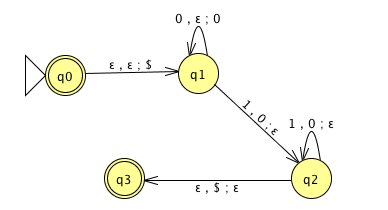
\includegraphics[height=100pt]{resources/machines/Lect9PDA.png}
    
    
    Draw the state diagram of a PDA with $\Sigma \cap \Gamma = \emptyset$.
    
\end{multicols}
    
\vspace{60pt}
    
A PDA recognizing the set $\{ \hspace{1.5 in} \}$ can be informally described as:
\begin{quote}
    Read symbols from the input. As each 0 is read, push it onto the stack. As soon as 1s are seen, pop a 0 off the stack for each 1 read. If the stack becomes empty and there is exactly one 1 left to read, read that 1 and accept the input. If the stack becomes empty and there are either zero or more than one 1s left to read, or if the 1s are finished while the stack still contains 0s, or if any 0s appear in the input following 1s, reject the input.
\end{quote}
    
    State diagram for this  PDA:

    
\vfill
\newpage
Consider the state diagram of a PDA with input alphabet 
$\Sigma$ and stack alphabet $\Gamma$.

\begin{center}
\begin{tabular}{|c|c|}
\hline
Label & means \\
\hline
$a, b ; c$ when $a \in \Sigma$, $b\in \Gamma$, $c \in \Gamma$ 
& \hspace{3in} \\
& \\
&\\
\hline
$a, \varepsilon ; c$ when $a \in \Sigma$, $c \in \Gamma$ 
& \hspace{3in} \\
& \\
&\\
\hline
$a, b ; \varepsilon$ when $a \in \Sigma$, $b\in \Gamma$
& \hspace{3in} \\
& \\
&\\
\hline
$a, \varepsilon ; \varepsilon$ when $a \in \Sigma$
& \hspace{3in} \\
& \\
&\\
\hline
\end{tabular}
\end{center}


How does the meaning change if $a$ is replaced by $\varepsilon$?

{\it Note: alternate notation is to replace $;$ with $\to$}


For the PDA state diagrams below, $\Sigma = \{0,1\}$.


\begin{center}
\begin{tabular}{c c}
Mathematical description of language & State diagram of PDA recognizing language\\
\hline
& 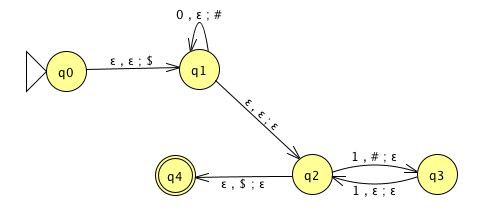
\includegraphics[width=3.5in]{resources/machines/Lect10PDA1.png}\\
\hline
& 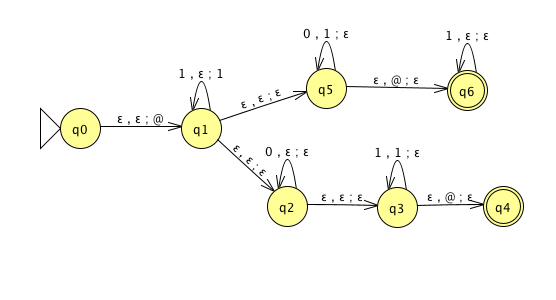
\includegraphics[width=3.5in]{resources/machines/Lect10PDA2.png}\\
\hline
& \\
$\{ 0^i 1^j 0^k \mid i,j,k \geq 0 \}$ & \\
\end{tabular}
\end{center}
 \vfill
\section*{Week3 friday}



{\bf Theorem}: For an alphabet $\Sigma$, For each language $L$ over $\Sigma$, 
\begin{center}
$L$ is recognized by some DFA \\
iff\\
$L$ is recognized by some NFA\\
iff\\
$L$ is described by some regular expression
\end{center}
If (any, hence all) these conditions apply, $L$ is called {\bf regular}.



{\bf Prove or Disprove}: There is some alphabet $\Sigma$ for which there is 
some language recognized by an NFA but not by any DFA.

\vspace{30pt}

{\bf Prove or Disprove}: There is some alphabet $\Sigma$ for which there is 
some finite language not described by any regular expression over $\Sigma$.

\vspace{30pt}


{\bf Prove or Disprove}: If a language is recognized by an NFA 
then the complement of this language is not recognized by any DFA.

\vspace{30pt}


\newpage
\begin{center}
\begin{tabular}{c|c}
Set & Cardinality \\
\hline
& \\
$\{0,1\}$ & \\
& \\
$\{0,1\}^*$ & \\
& \\
$\mathcal{P}( \{0,1\})$ & \\
& \\
The set of all languages over $\{0,1\}$ & \\
& \\
The set of all regular expressions over $\{0,1\}$ & \\
& \\
The set of all regular languages over $\{0,1\}$ & \\
& \\
\end{tabular}
\end{center}



\vfill

\newpage

{\bf Pumping Lemma} (Sipser Theorem 1.70): If $A$ is a regular language, then there
is a number $p$ (a {\it pumping length}) where, if $s$ is any string in $A$ of length at least $p$, 
then $s$ may be divided into three pieces, $s = xyz$ such that
\vspace{-10pt}
\begin{itemize}
\item $|y| > 0$
\item for each $i \geq 0$, $xy^i z \in A$
\item $|xy| \leq p$.
\end{itemize}


{\bf True or False}: A pumping length for $A = \{ 0,1 \}^*$ is $p = 5$.

\vspace{100pt}

{\bf True or False}: A pumping length for $A = \{1, 01, 001, 0001, 00001 \}$ is $p = 4$.

\vspace{100pt}

{\bf True or False}: A pumping length for $A = \{0^j 1 \mid  j \geq 0 \}$ is $p = 3$.


\vspace{100pt}

{\bf True or False}: For any language $A$, if $p$  is a  pumping length for $A$ and $p' > p$,  then 
$p'$ is also a pumping length for $A$.
 \vfill
\end{document}